\documentclass[conference]{IEEEtran}
\IEEEoverridecommandlockouts
\usepackage{cite}
\usepackage{amsmath,amssymb,amsfonts}
\usepackage{algorithmic}
\usepackage{graphicx}
\usepackage{textcomp}
\usepackage{xcolor}
\usepackage{booktabs}
\usepackage{float}
\usepackage{cuted}
\usepackage{capt-of}
\usepackage[hidelinks]{hyperref}

\def\BibTeX{{\rm B\kern-.05em{\sc i\kern-.025em b}\kern-.08em
    T\kern-.1667em\lower.7ex\hbox{E}\kern-.125emX}}

\begin{document}

\title{Multi-Scale Hybrid Attention and Equalization for Skin Lesion Segmentation}

\author{
\IEEEauthorblockN{Jinkun Wang*}
\IEEEauthorblockA{\textit{School of Computer Science} \\
\textit{Northwestern Polytechnical University}\\
Xi'an, China \\
wangjinkun@mail.nwpu.edu.cn}
\and
\IEEEauthorblockN{Xuanhe Wang}
\IEEEauthorblockA{\textit{School of Physics} \\
\textit{Zhengzhou University}\\
Zhengzhou, China \\
wxh1206@stu.zzu.edu.cn}
}

\maketitle

\begin{abstract}
Skin lesion segmentation in dermoscopy remains difficult because lesion size and appearance vary widely, and the image quality is often degraded by low contrast, uneven illumination, and hair occlusion. This paper builds on a nested encoder-decoder baseline and adds three lightweight modifications aimed at common failure cases in this setting: histogram equalization before encoding, hybrid attention after encoder and decoder convolutions, and multi-scale fusion at the bottleneck. On ISIC 2018, the resulting model reaches a Dice score of 88.34 percent and an intersection-over-union score of 79.73 percent, improving over the baseline by 1.96 and 2.95 percentage points. The ablation study shows that contrast enhancement contributes the largest single gain, while attention and bottleneck fusion provide smaller additional improvements.
\end{abstract}

\begin{IEEEkeywords}
skin lesion segmentation, attention mechanism, histogram equalization, multi-scale fusion
\end{IEEEkeywords}

\section{Introduction}

Automated segmentation of skin lesions from dermoscopic images is a prerequisite for computer-aided melanoma diagnosis. Manual annotation is time-consuming, error-prone, and subject to substantial inter-observer variability. The ISIC 2018 challenge~\cite{codella2018,tschandl2018} provides a standardized benchmark of 2,594 training images, driving significant progress in deep learning-based skin lesion segmentation.

Since the introduction of U-Net~\cite{ronneberger2015}, encoder-decoder models have remained the main workhorse for this task because they offer reliable localization without excessive computational cost. UNet++~\cite{zhou2018} improved this family through nested skip pathways and deep supervision, and it is already a strong baseline for dermoscopic segmentation. Even so, several failure modes remain common in practice. Low-contrast boundaries are still hard to recover, while hair, specular streaks, and surrounding skin texture may be propagated through the skip pathway as false positive evidence.

These errors do not arise in the same way. In some cases the lesion boundary is weak from the input stage, so later decoding can only refine incomplete evidence. In others the lesion is coarsely localized, but thin artifacts and background texture remain active in intermediate features. Large or diffuse lesions introduce another difficulty because local decoding alone does not always enforce broad contour consistency. For this reason, the UNet++ backbone is left unchanged and three surrounding stages are modified: histogram equalization (HE) on the LAB luminance channel before encoding, a hybrid attention block (HA) after each encoder and decoder DoubleConv block, and a multi-scale fusion block (MSF) at the bottleneck. Figure~\ref{fig:hardcases} shows the type of examples behind this design.

\begin{figure}[htbp]
\centering
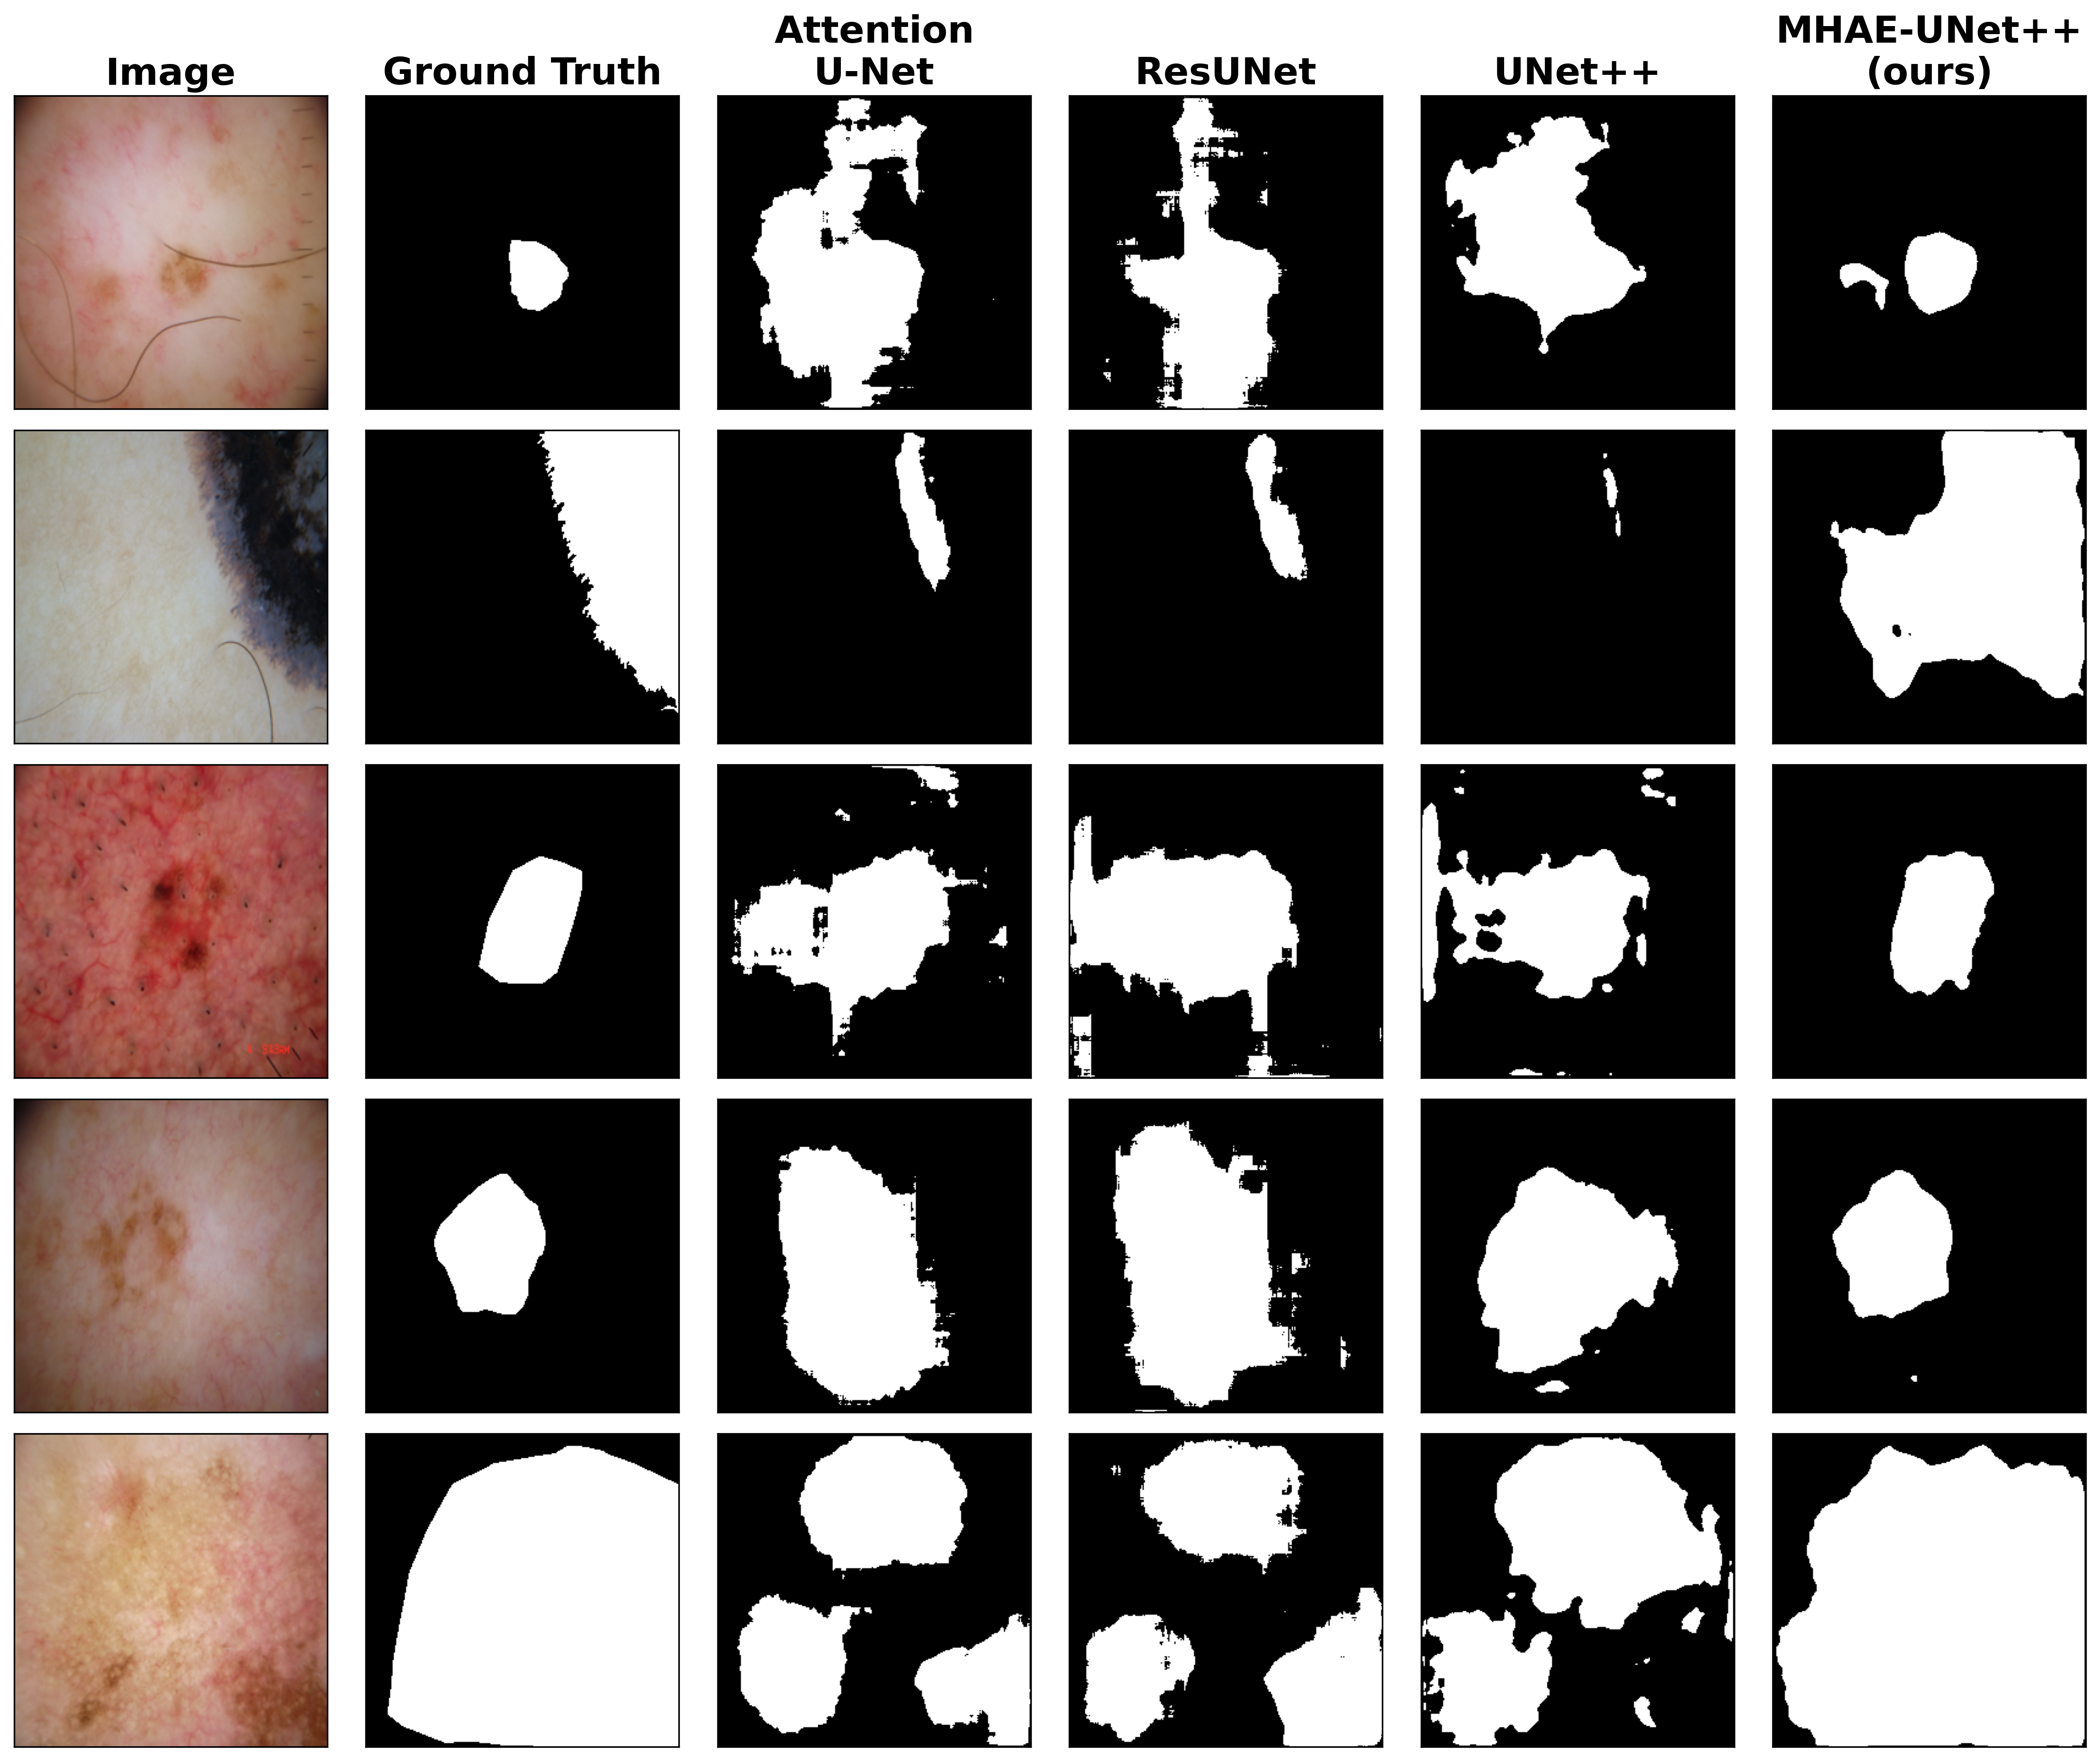
\includegraphics[width=\columnwidth]{figures/fig1_comparison.png}
\caption{Challenging examples.}
\label{fig:hardcases}
\end{figure}

The scope of the paper is intentionally narrow. The goal is not to replace UNet++ with a heavier architecture, but to test how far a strong baseline can be improved by correcting a small number of recurring task-specific errors. The resulting model reaches 88.34\% Dice and 79.73\% IoU on ISIC 2018. The ablation is included mainly to show which parts of the modification matter most for this dataset.

\section{Related Work}

\subsection{Encoder-Decoder Architectures for Medical Segmentation}

U-Net~\cite{ronneberger2015} established the encoder-decoder paradigm with symmetric skip connections, and its variants have since proliferated. Attention U-Net~\cite{oktay2018} introduced gated attention at skip connections to suppress irrelevant features. ResUNet~\cite{zhang2018} adopted residual connections for deeper gradient propagation. UNet++~\cite{zhou2018} redesigned skip pathways as a nested dense structure with deep supervision, enabling multi-level feature aggregation. MALUNet~\cite{ruan2022} proposed a lightweight multi-attention design specifically for skin lesions, whereas transformer-based approaches~\cite{chen2021transunet} and foundation model adaptation~\cite{ma2024medsam} have also been explored at higher computational cost.

Despite this breadth of work, the design choices reflect different assumptions about where the main bottleneck lies. Attention U-Net mainly targets skip-level feature selection, which is useful when encoder features are informative but incompletely filtered. Transformer-based methods widen contextual modeling much more aggressively, but their gain comes with heavier memory use and training cost, which is not always justified for a single-modality benchmark of this size. MALUNet moves in the opposite direction by emphasizing compactness. For the present study, UNet++ is a suitable starting point because it already supplies dense cross-scale communication; the remaining problem is less about missing skip connections than about how noisy local evidence, weak contrast, and limited deep context interact in the same prediction path.

\subsection{Attention Mechanisms for Feature Refinement}

Channel-wise attention~\cite{hu2018} recalibrates feature responses, whereas spatial attention suppresses visually distracting regions. CBAM~\cite{woo2018} combines the two sequentially and remains attractive because it provides a clear and inexpensive intervention on intermediate features. This matters in dermoscopy, where nuisance responses often appear as feature families associated with hair edges, illumination streaks, or coarse background texture rather than as isolated pixels.

\subsection{Multi-Scale Feature Aggregation}

Pyramid pooling~\cite{zhao2017} and ASPP~\cite{chen2018} both address the need for multi-scale context. This issue is especially pertinent in dermoscopy, where the same semantic label may correspond either to a compact high-contrast lesion or to a diffuse weakly bounded region. Their difference is not only structural but also practical. Multi-scale aggregation is most useful once the representation has become semantic enough to benefit from larger context. Applying strong context mixing too early can blur local border evidence that shallow layers still need to preserve. Bottleneck-level aggregation is therefore a natural location for introducing additional scale diversity without repeatedly perturbing shallow texture features.

\subsection{Preprocessing in Dermoscopy}

Dermoscopy has long relied on preprocessing because some failure modes start before the network sees the image. CLAHE~\cite{zuiderveld1994} is particularly attractive here because it improves local luminance contrast without heavily distorting global structure, and prior work has shown that contrast enhancement can improve dermoscopic lesion segmentation~\cite{schaefer2011}. If the contrast around the lesion edge is already compressed in the input, later feature refinement has little chance to recover it reliably.

\section{Method}

UNet++~\cite{zhou2018} is used as the baseline because its nested skip pathways already provide strong feature propagation and dense cross-scale interaction. The remaining limitations appear in three places: poorly contrasted inputs, intermediate features affected by distracting image patterns, and deep features with limited receptive-field diversity. MHAE-UNet++ addresses these three issues through HE before encoding, HA during feature transformation, and MSF at the bottleneck. The overall architecture is shown in Fig.~\ref{fig:fullmodule}.

\begin{strip}
\centering
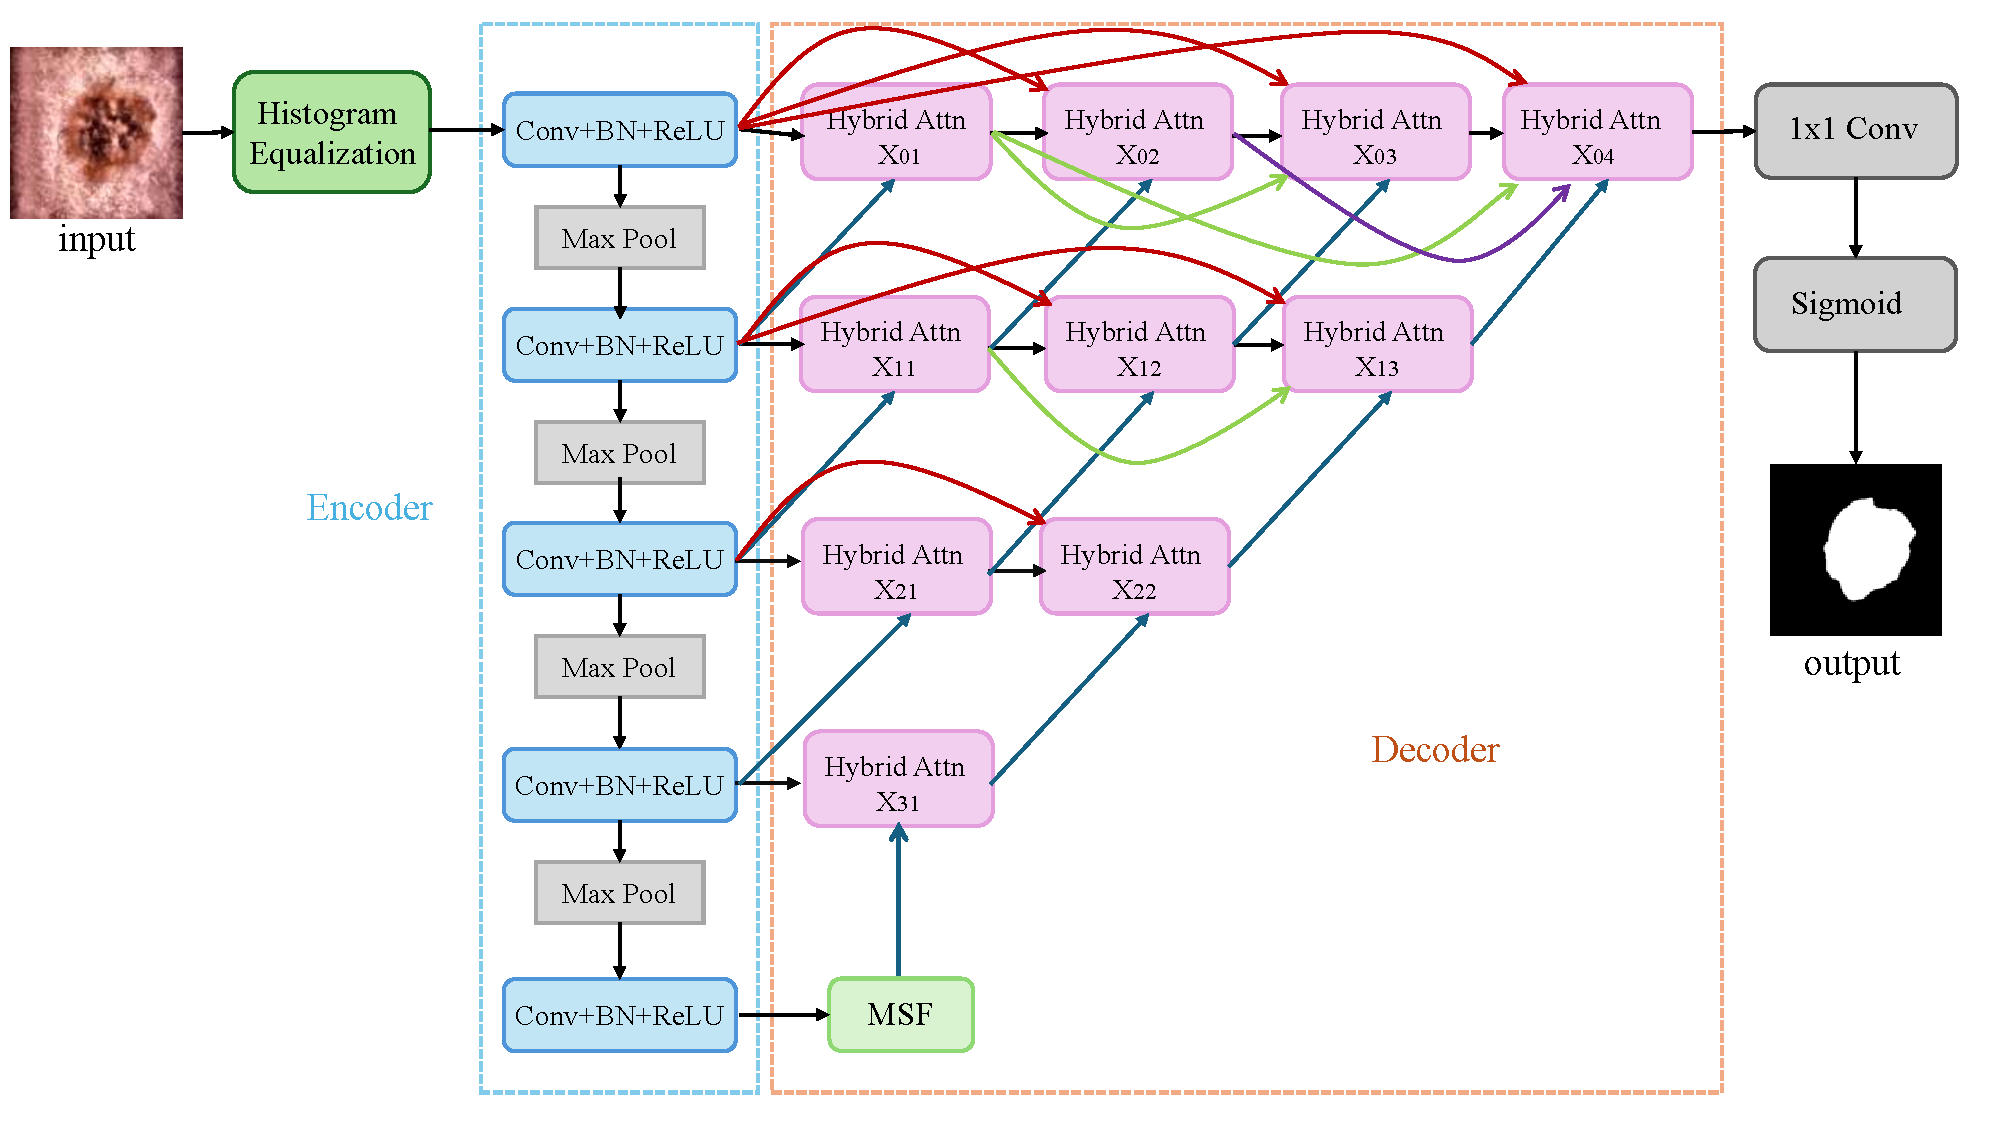
\includegraphics[width=0.70\textwidth]{figures/Full Module.pdf}
\captionof{figure}{Overall architecture of MHAE-UNet++.}
\label{fig:fullmodule}
\end{strip}

\subsection{Baseline: UNet++}

UNet++ consists of five encoder stages with channel dimensions $[32,64,128,256,512]$. Each stage applies two $3\times3$ convolutions followed by batch normalization and ReLU, with $2\times2$ max pooling between stages. Its key distinction from U-Net lies in the nested skip design: node $X^{i,j}$ aggregates the upsampled output of $X^{i+1,j-1}$ together with all preceding shallower nodes $X^{i,0},\dots,X^{i,j-1}$ before another double-convolution transformation. This dense skip formulation reduces the semantic gap between encoder and decoder representations and provides the reference topology on which the proposed modules are built.

\subsection{Hybrid Attention Module}

The HA module is used to suppress unstable responses in intermediate feature maps. In dermoscopic images, textured healthy skin, illumination streaks, and hairs often produce strong activations even though they are not part of the lesion. HA is therefore inserted after every encoder and decoder DoubleConv block so that feature maps are adjusted immediately after local evidence is formed. As illustrated in Fig.~\ref{fig:ha}, the module applies channel attention first and spatial attention second. For a feature map $\mathbf{F}\in\mathbb{R}^{C\times H\times W}$, the channel attention $\mathbf{M}_c\in\mathbb{R}^{C\times1\times1}$ pools global evidence through both average and max statistics and maps them through a shared MLP with reduction ratio 16. The spatial attention $\mathbf{M}_s\in\mathbb{R}^{1\times H\times W}$ then operates on cross-channel average and max pooling maps followed by a $7\times7$ convolution. Formally:

\begin{equation}
\begin{aligned}
\mathbf{F}_{\text{c}} &= \mathbf{M}_c(\mathbf{F}) \otimes \mathbf{F}, \\
\mathbf{F}' &= \mathbf{M}_s(\mathbf{F}_{\text{c}}) \otimes \mathbf{F}_{\text{c}}.
\end{aligned}
\end{equation}

This ordering is adopted because the unstable responses in dermoscopy are often organized channel-wise before they are clearly separable spatially. After convolution, hairs and specular highlights can dominate several channels as high-response edge patterns. Channel recalibration first reduces such feature families at the descriptor level; spatial attention then acts on a cleaner map and is less likely to preserve thin background structures around the lesion. This is particularly relevant in decoder stages, where false activations can otherwise be expanded together with genuine lesion regions. The module adds approximately 60K parameters to the 9.16M baseline.

\begin{figure}[htbp]
\centering
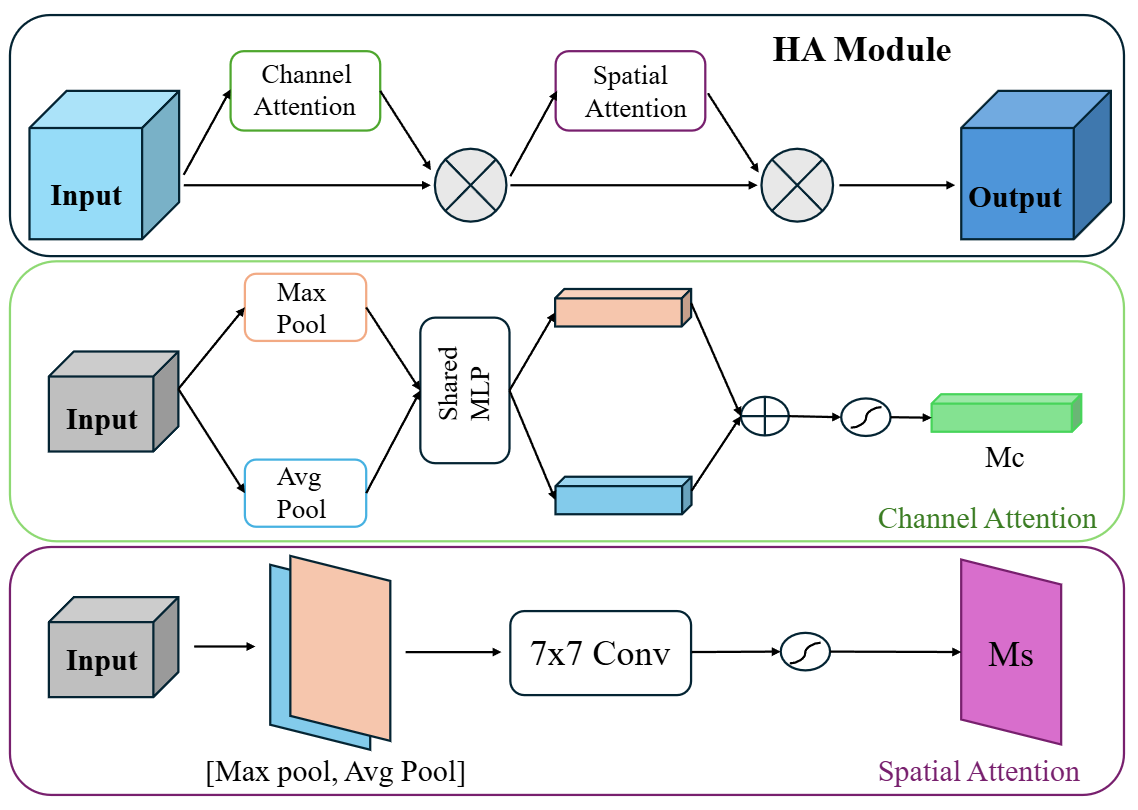
\includegraphics[width=0.94\columnwidth]{figures/HA Module.png}
\caption{HA module.}
\label{fig:ha}
\end{figure}

\subsection{Multi-Scale Fusion Module}

Even with nested skip connections, UNet++ processes each scale using a limited effective receptive field at a given depth. This becomes problematic when lesion interpretation depends on balancing local border sharpness against broader structural context. MSF is therefore placed at the bottleneck ($16\times16$ resolution, 512 channels), where semantic abstraction is high and scale mixing is most valuable. This placement is deliberate. Shallow stages are still dominated by texture fidelity and edge localization; forcing heavy multi-scale mixing there can wash out weak but useful border cues and make decoder recovery harder. At the bottleneck, the representation is already compressed and semantically stronger, so the main missing information is not fine texture but context range. In practice, this module is meant to complement rather than replace the dense skip aggregation already present in UNet++. As illustrated in Fig.~\ref{fig:msf}, MSF follows the ASPP principle of parallel context extraction through four $3\times3$ dilated convolutions with rates 1, 6, 12, and 18, together with a global average pooling branch. Each branch produces 128 channels; the resulting descriptors are concatenated and compressed by a $1\times1$ fusion layer with batch normalization and ReLU to restore a 512-channel output.

\begin{figure}[htbp]
\centering
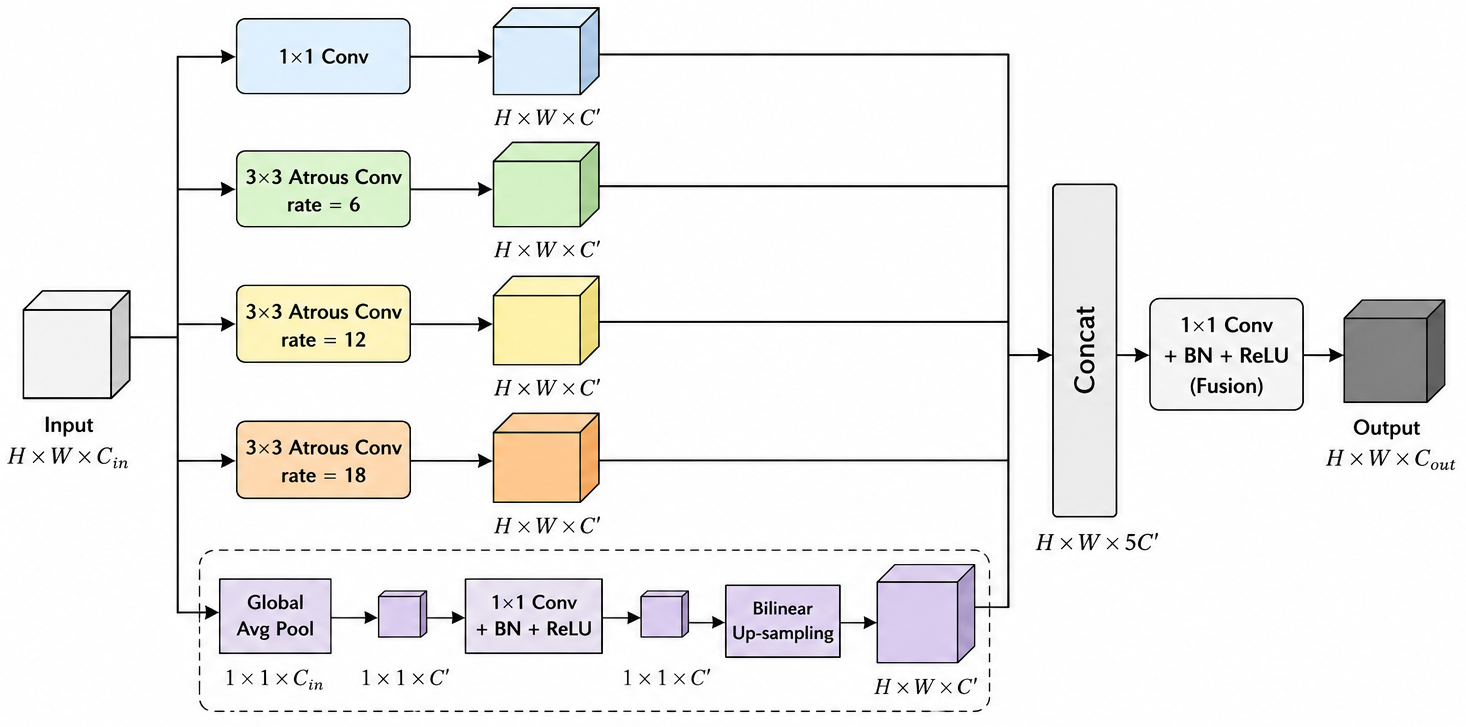
\includegraphics[width=0.94\columnwidth]{figures/MSF Module.png}
\caption{MSF module.}
\label{fig:msf}
\end{figure}

\subsection{Histogram Equalization Module}

The HE module addresses the degradation of boundary evidence at the input level. When the luminance structure is weak, subsequent feature refinement has limited information to recover. Consequently, contrast enhancement is applied before both training and inference by operating only on the L-channel of the LAB color space:

\begin{equation}
\begin{aligned}
\mathbf{I}_{\text{LAB}} &= \text{RGB2LAB}(\mathbf{I}), \\
\mathbf{I}_{\text{LAB}}[:,:,0] &= \text{CLAHE}(\mathbf{I}_{\text{LAB}}[:,:,0] / 100) \times 100, \\
\mathbf{I}_{\text{enhanced}} &= \text{LAB2RGB}(\mathbf{I}_{\text{LAB}}).
\end{aligned}
\end{equation}

Only the L-channel is equalized because lesion chromatic patterns remain diagnostically relevant and also serve as segmentation cues. Direct equalization in RGB space can shift color relationships between lesion and surrounding skin, especially in reddish or brown-toned cases where subtle chromatic transitions already carry boundary information. Processing luminance alone improves local contrast while leaving the chromatic distribution largely intact. This makes the preprocessing easier to combine with a standard ImageNet-initialized encoder, since the color statistics are perturbed less aggressively than under full RGB equalization. We use a clip limit of 0.02 with automatically determined kernel size. The enhanced images are pre-computed and cached to disk to decouple this signal-level intervention from training-time stochasticity.

\subsection{Training Configuration}

All models are trained with a combined Binary Cross-Entropy and Dice loss to balance pixel-wise calibration with overlap quality:

\begin{equation}
\mathcal{L} = 0.5 \cdot \mathcal{L}_{\text{BCE}} + 0.5 \cdot \mathcal{L}_{\text{Dice}}.
\end{equation}

Images are resized to $256\times256$ and normalized using ImageNet statistics. Data augmentation includes random horizontal and vertical flips, rotation ($\pm 15^\circ$), and brightness and contrast jittering. We use the AdamW optimizer with learning rate $1\times10^{-4}$, weight decay $1\times10^{-5}$, and batch size 8 with automatic mixed precision. Training proceeds for 50 epochs with a linear warmup of 3 epochs followed by cosine annealing.

\section{Experiments and Results}

\subsection{Dataset and Implementation}

Experiments are conducted on the ISIC 2018 skin lesion segmentation benchmark~\cite{codella2018,tschandl2018}, which exhibits substantial variation in lesion size, color distribution, and boundary clarity. The split used in this study comprises 2,594 training images, 100 validation images, and 1,000 test images with binary ground-truth masks. The official validation set is used for model selection, and final performance is reported on the test set.

\subsection{Evaluation Metrics}

We report two standard segmentation metrics:

\begin{equation}
\text{DSC} = \frac{2|P \cap G|}{|P| + |G|},
\end{equation}
\begin{equation}
\text{IoU} = \frac{|P \cap G|}{|P \cup G|},
\end{equation}

where $P$ and $G$ denote predicted and ground truth binary masks.

\subsection{Comparison with Baseline Methods}

Table~\ref{tab:comparison} summarizes the comparison with representative convolutional baselines. MHAE-UNet++ improves upon all three reference architectures. The key comparison is with UNet++, since that is the backbone modified in this work. Relative to this baseline, the proposed model gains 1.96 percentage points in Dice and 2.95 points in IoU. The larger gain in IoU is consistent with the type of errors being reduced. Dice is relatively tolerant to small peripheral disagreements when the lesion core is already segmented reasonably well, whereas IoU is more sensitive to extra foreground fragments and boundary spillover. In this dataset, many baseline errors come from residual activations around lesion edges and thin artifact responses. Cleaning those regions changes the union term more visibly, so IoU benefits slightly more than Dice. The gap between the two improvements also suggests that the gain is not mainly from filling large missing regions, but from reducing boundary overreach and scattered false positives.

\begin{table}[!t]
\centering
\caption{Baseline comparison on ISIC 2018.}
\label{tab:comparison}
\begin{tabular*}{\columnwidth}{@{\extracolsep{\fill}}lcc@{}}
\toprule
\textbf{Model} & \textbf{DSC (\%)} & \textbf{IoU (\%)} \\
\midrule
Attention U-Net~\cite{oktay2018} & 86.51 & 76.95 \\
ResUNet~\cite{zhang2018}         & 86.31 & 76.72 \\
UNet++~\cite{zhou2018}           & 86.38 & 76.78 \\
\midrule
\textbf{MHAE-UNet++ (ours)} & \textbf{88.34} & \textbf{79.73} \\
\bottomrule
\end{tabular*}
\end{table}

\subsection{Ablation Study}

To determine how each component contributes, HE, HA, and MSF are added incrementally to the UNet++ baseline. The corresponding results are listed in Table~\ref{tab:ablation}. The question here is simple: which parts of the modification carry most of the gain on this dataset.

Table~\ref{tab:ablation} shows a fairly direct pattern. HE produces the largest standalone gain (+1.39 Dice), which fits the low-contrast boundaries seen in many ISIC images. This is also where the intervention is applied earliest. Once the lesion contour is weak in the input, later refinement blocks can only work with incomplete evidence. Improving luminance contrast before feature extraction therefore has a broader downstream effect than a later module acting on already degraded features. HA alone adds +0.61 Dice, so the attention block still helps without preprocessing changes. The HA + HE setting reaches 88.14\%, which is higher than either module alone.

\begin{table}[htbp]
\centering
\caption{Ablation results on ISIC 2018.}
\label{tab:ablation}
\begin{tabular*}{\columnwidth}{@{\extracolsep{\fill}}lcc@{}}
\toprule
\textbf{Configuration} & \textbf{DSC (\%)} & \textbf{IoU (\%)} \\
\midrule
UNet++ (baseline)      & 86.38 & 76.78 \\
+ HE                  & 87.77 & 78.85 \\
+ HA                  & 86.99 & 77.84 \\
+ HA + MSF            & 87.07 & 77.99 \\
+ HA + HE             & 88.14 & 79.53 \\
\midrule
\textbf{MHAE-UNet++ (full)} & \textbf{88.34} & \textbf{79.73} \\
\bottomrule
\end{tabular*}
\end{table}

MSF contributes a smaller gain when added without HE, increasing HA + MSF to 87.07\%. This more limited gain is plausible for the current backbone. UNet++ already performs dense cross-scale aggregation through its skip design, so the bottleneck is not devoid of contextual support. The MSF block supplements that context with explicit receptive-field diversity, but the room left for improvement is narrower than for input contrast correction. This is also compatible with the lesion characteristics in ISIC 2018: many difficult cases are dominated by weak boundaries and thin artifacts rather than by complete failure of global localization. In the full configuration, MSF raises performance from 88.14\% (HA + HE) to 88.34\%. The pattern is therefore additive but uneven: early boundary recovery matters most, feature reweighting gives a stable refinement, and extra bottleneck context provides a smaller final adjustment. No module addition reduces performance in the reported settings.

Figure~\ref{fig:bestcases} provides additional qualitative examples. Across lesions with different scales, shapes, and boundary characteristics, the predicted masks show smoother contours and fewer fragmented foreground regions. Thin artifact responses outside the lesion are reduced, which matches the intended role of HA in suppressing distracting activations. For lesions with diffuse margins, the masks also appear more spatially consistent instead of breaking into small local protrusions. The visual changes are modest at first glance, but they align with the observed IoU gain, which is where boundary cleaning and false-positive suppression are reflected more directly.

\begin{figure}[htbp]
\centering
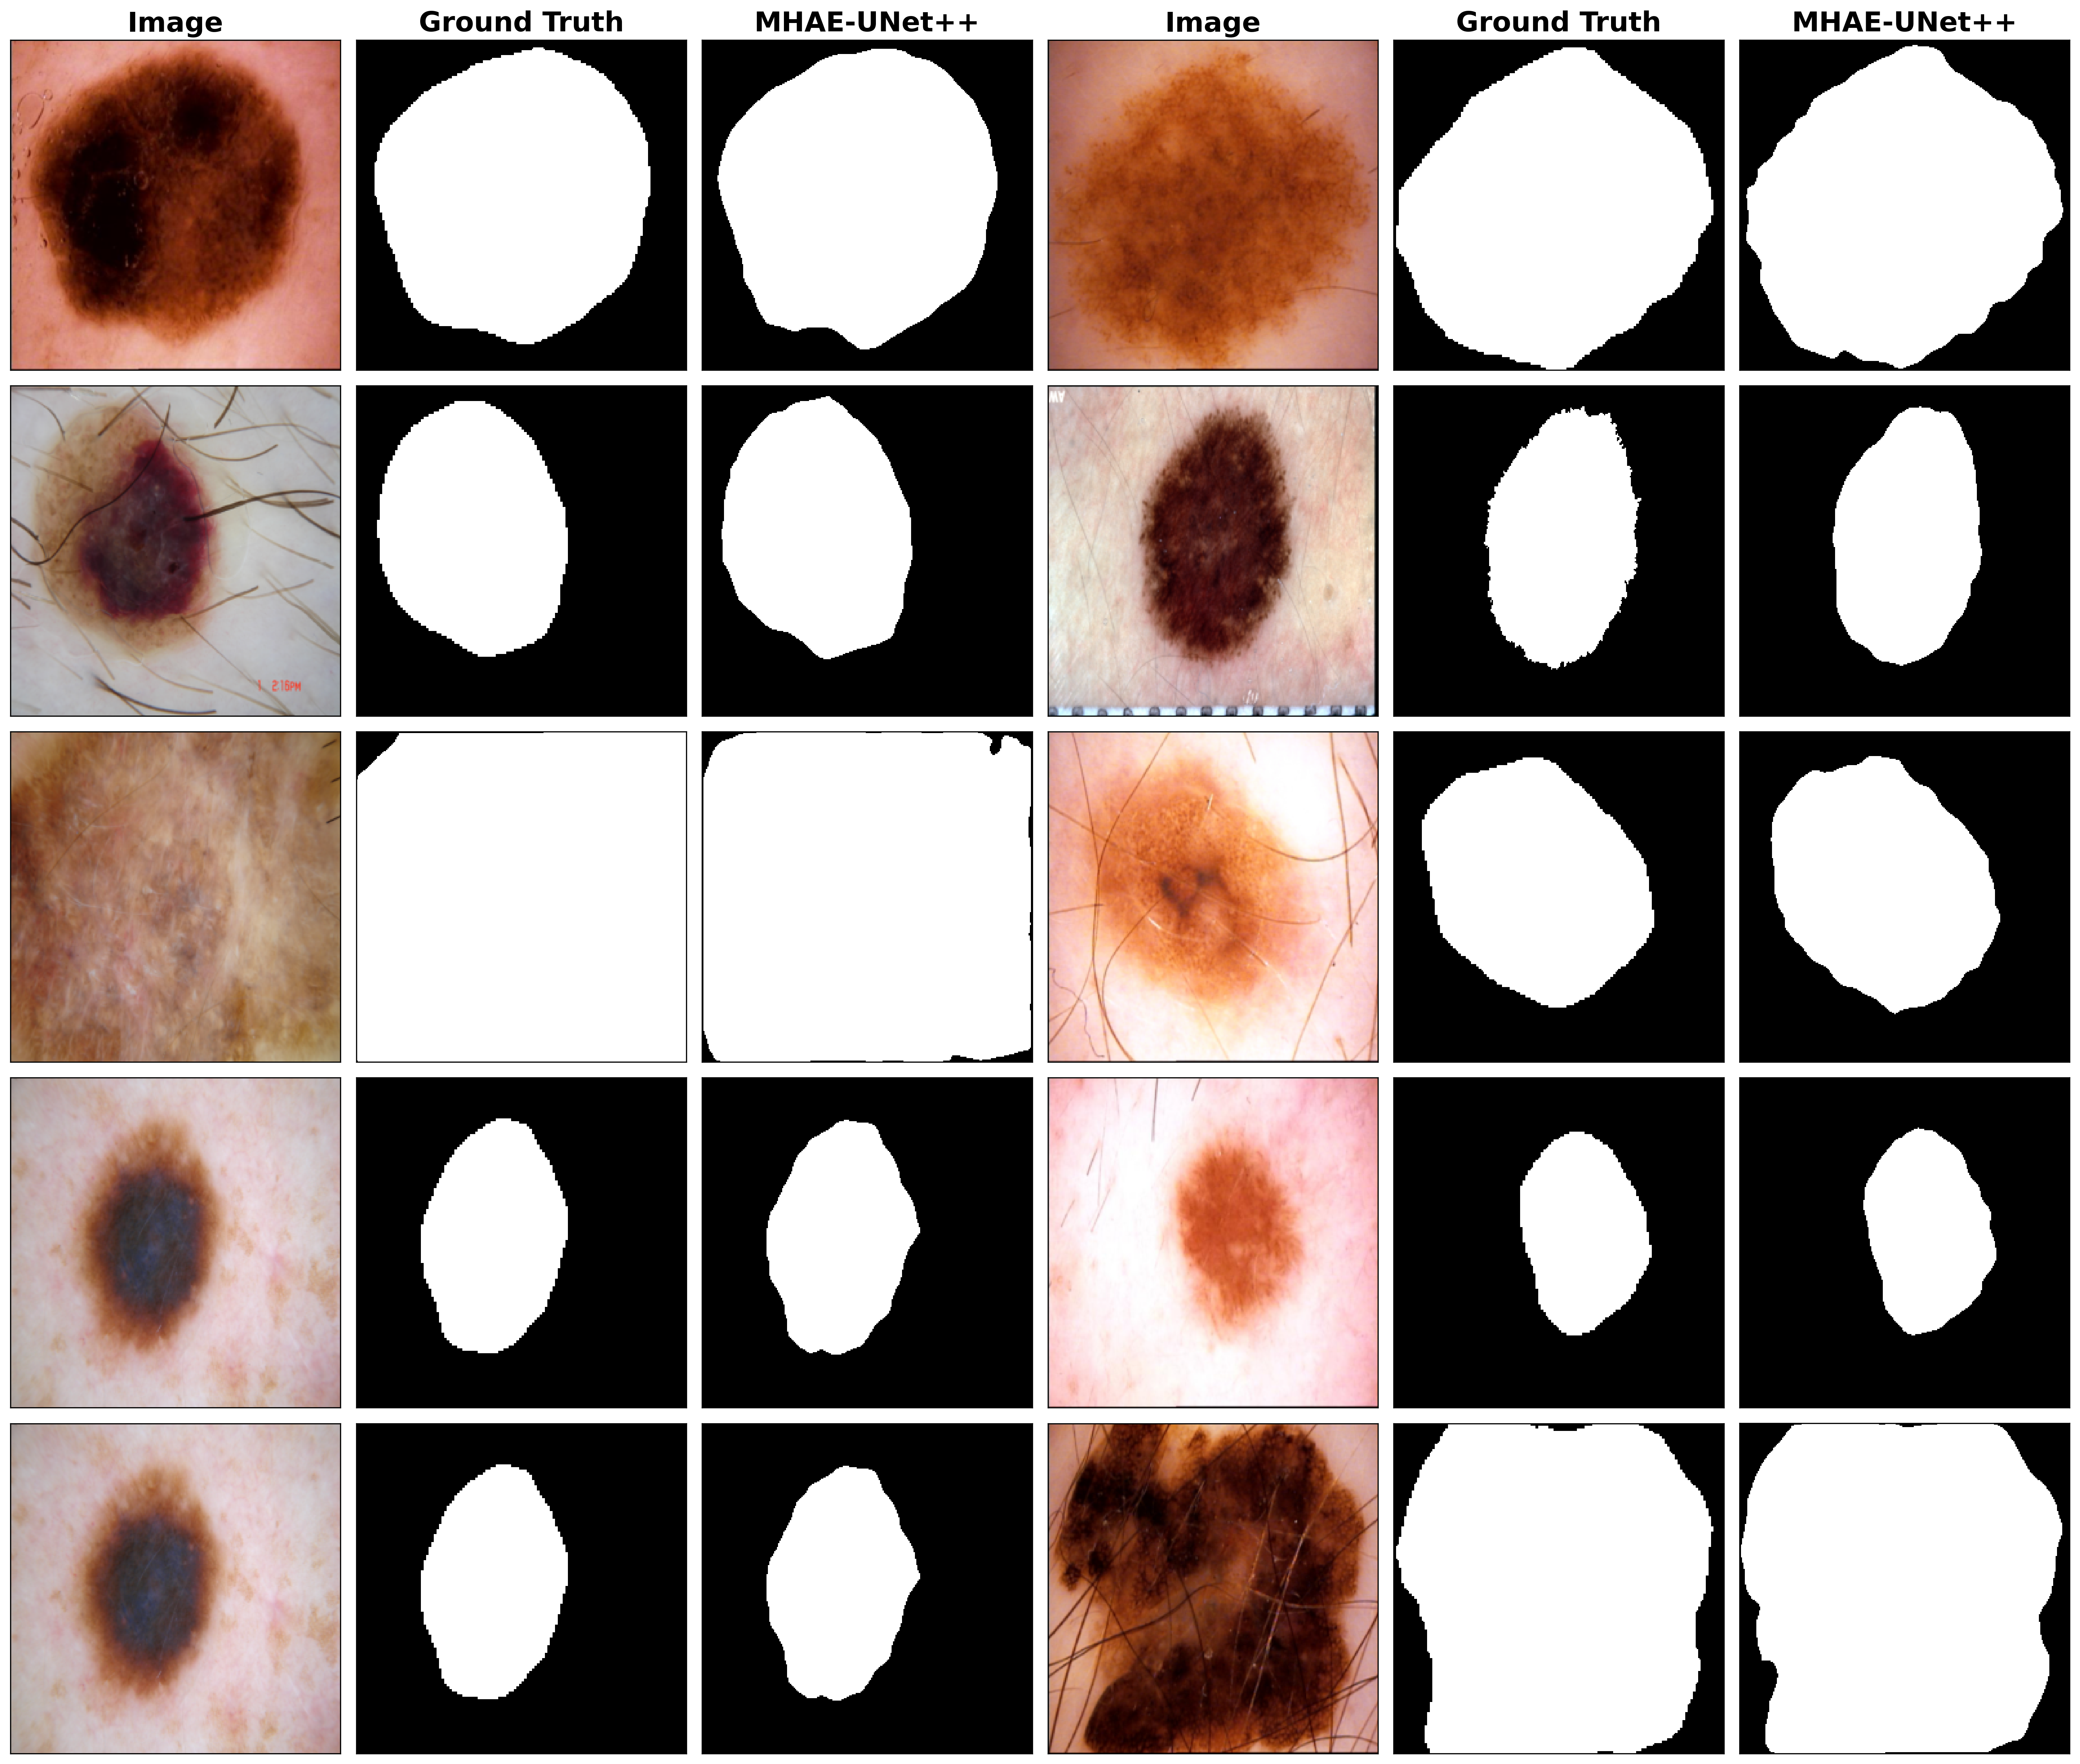
\includegraphics[width=\columnwidth]{figures/fig2_best10.png}
\caption{Qualitative segmentation examples.}
\label{fig:bestcases}
\end{figure}

\section{Conclusion}

The results show that UNet++ still leaves room for improvement on ISIC 2018 without requiring a change of backbone. MHAE-UNet++ addresses weak boundary contrast, distracting background patterns, and limited receptive-field variation while keeping the encoder-decoder structure unchanged. This design improves UNet++ from 86.38\% to 88.34\% Dice and from 76.78\% to 79.73\% IoU. The ablation results indicate that the largest gain comes from input-side contrast correction, while attention and bottleneck fusion act mainly as incremental refinements on top of a stronger input signal.

The present design still has clear limits. HE is fixed preprocessing and does not adapt during optimization. The module settings were tuned for ISIC 2018, and the current evidence is restricted to a single benchmark, leaving cross-dataset robustness unresolved.

\begin{thebibliography}{00}

\bibitem{codella2018}
N.~Codella, V.~Rotemberg, P.~Tschandl, M.~E.~Celebi, S.~Dusza, D.~Gutman, B.~Helba, A.~Kalloo, K.~Liopyris, M.~Marchetti, H.~Kittler, and A.~Halpern,
``Skin lesion analysis toward melanoma detection 2018: A challenge hosted by the International Skin Imaging Collaboration (ISIC),''
arXiv:1902.03368, 2019. [Online]. Available: \url{https://arxiv.org/abs/1902.03368}

\bibitem{tschandl2018}
P.~Tschandl, C.~Rosendahl, and H.~Kittler,
``The HAM10000 dataset, a large collection of multi-source dermatoscopic images of common pigmented skin lesions,''
\textit{Scientific Data}, vol.~5, Art.~no.~180161, 2018.

\bibitem{ronneberger2015}
O.~Ronneberger, P.~Fischer, and T.~Brox,
``U-Net: Convolutional networks for biomedical image segmentation,''
in \textit{Proc. MICCAI}, 2015, pp.~234--241.

\bibitem{zhou2018}
Z.~Zhou, M.~M.~R.~Siddiquee, N.~Tajbakhsh, and J.~Liang,
``UNet++: A nested U-Net architecture for medical image segmentation,''
in \textit{Deep Learn. Med. Image Anal. Multimodal Learn. Clin. Decis. Support}, 2018, pp.~3--11.

\bibitem{oktay2018}
O.~Oktay, J.~Schlemper, L.~Le~Folgoc, M.~Lee, M.~Heinrich, K.~Misawa, K.~Mori, S.~McDonagh, N.~Y.~Hammerla, B.~Kainz, B.~Glocker, and D.~Rueckert,
``Attention U-Net: Learning where to look for the pancreas,''
arXiv:1804.03999, 2018.

\bibitem{zhang2018}
Z.~Zhang, Q.~Liu, and Y.~Wang,
``Road extraction by deep residual U-Net,''
\textit{IEEE Geosci. Remote Sens. Lett.}, vol.~15, no.~5, pp.~749--753, 2018.

\bibitem{ruan2022}
J.~Ruan, S.~Xiang, M.~Xie, T.~Liu, and Y.~Fu,
``MALUNet: A multi-attention and light-weight UNet for skin lesion segmentation,''
in \textit{Proc. IEEE Int. Conf. Bioinf. Biomed.}, 2022, pp.~1150--1156.

\bibitem{chen2021transunet}
J.~Chen, Y.~Lu, Q.~Yu, X.~Luo, E.~Adeli, Y.~Wang, L.~Lu, A.~L.~Yuille, and Y.~Zhou,
``TransUNet: Transformers make strong encoders for medical image segmentation,''
arXiv:2102.04306, 2021.

\bibitem{ma2024medsam}
J.~Ma, Y.~He, F.~Li, L.~Han, C.~You, and B.~Wang,
``Segment anything in medical images,''
\textit{Nature Communications}, vol.~15, Art.~no.~654, 2024.

\bibitem{hu2018}
J.~Hu, L.~Shen, and G.~Sun,
``Squeeze-and-excitation networks,''
in \textit{Proc. CVPR}, 2018, pp.~7132--7141.

\bibitem{woo2018}
S.~Woo, J.~Park, J.-Y.~Lee, and I.~S.~Kweon,
``CBAM: Convolutional block attention module,''
in \textit{Proc. ECCV}, 2018, pp.~3--19.

\bibitem{zhao2017}
H.~Zhao, J.~Shi, X.~Qi, X.~Wang, and J.~Jia,
``Pyramid scene parsing network,''
in \textit{Proc. CVPR}, 2017, pp.~2881--2890.

\bibitem{chen2018}
L.-C.~Chen, Y.~Zhu, G.~Papandreou, F.~Schroff, and H.~Adam,
``Encoder-decoder with atrous separable convolution for semantic image segmentation,''
in \textit{Proc. ECCV}, 2018, pp.~833--851.

\bibitem{zuiderveld1994}
K.~Zuiderveld,
``Contrast limited adaptive histogram equalization,''
in \textit{Graphics Gems IV}. San Diego, CA, USA: Academic Press Professional, Inc., 1994, pp.~474--485.

\bibitem{schaefer2011}
G.~Schaefer, M.~I.~Rajab, M.~E.~Celebi, and H.~Iyatomi,
``Colour and contrast enhancement for improved skin lesion segmentation,''
\textit{Comput. Med. Imaging Graph.}, vol.~35, no.~2, pp.~99--104, 2011.

\end{thebibliography}

\end{document}
